% Welcome to the TeX source of Open Calculus.
% This source (and all material from opencalculus.org
% is licensed under a Creative Commons Attribution-NonCommercial-ShareAlike 3.0 Unported License.
% (http://creativecommons.org/licenses/by-nc-sa/3.0/deed.en_US)
%
% As always, please email me directly at dixon@opencalculus.org with any comments, questions, suggestions, or concerns!

\documentclass[oneside]{article}

\usepackage{amsmath}
\usepackage{anysize}
\usepackage{hyperref}
\usepackage{graphicx}

\marginsize{0.5in}{0.5in}{0.5in}{0.5in}

\linespread{1.1}

\begin{document}


\begin{titlepage}

\newcommand{\HRule}{\rule{\linewidth}{0.5mm}} 

\center

\textsc{\large \href{http://opencalculus.org}{opencalculus.org}}\\[1.5cm] 
\textsc{\Large \textit{A free, open-source text}}\\[0.5cm] 

\HRule \\[0.4cm]
{ \huge \bfseries Open Calculus}\\[0.4cm]
\HRule \\[1.5cm]

\Large \emph{Author:}\\
Dixon \textsc{Crews}\\[0.5cm]
\small \texttt{\href{mailto:dixon@opencalculus.org}{dixon@opencalculus.org}} \\ [3.5cm]

{\large Version 1.0}\\[1cm]
{\large December 2012}\\[3cm]

\vfill 

\end{titlepage}

\tableofcontents
\vfill

\section{Introduction}
\subsection{About this text}
\textbf{Welcome!} Before we start getting into the calculus portion of this book, I thought it would be best to introduce both myself and this text. My name is Dixon Crews and I'm a freshman at N.C. State University in Raleigh, North Carolina majoring in Computer Science. I'm also minoring in Music Performance with a concentration in piano. I was first introduced to calculus in my senior year of high school in an AP Calculus BC course. I have found the study and applications of calculus to be utterly fascinating, and I have also seen first hand the need for a free and open-source calculus text to aid those currently enrolled in a college-level math course.

On December 8, 2012, I registered \texttt{opencalculus.org} and began work on this very text. It should be apparent now that I am not an authority on all things math, and therefore this book should not be seen as the be all end all of calculus texts. Instead, we will approach the topics of college-level calculus courses with a reasonable but not exhaustive rigor that anyone may understand.

It should also be known that this is an \textit{ongoing, ever-changing} text. I welcome and encourage all suggestions, comments, and questions in the form of an email to \texttt{\href{mailto:dixon@opencalculus.org}{dixon@opencalculus.org}}. 

This text is licensed under a \href{http://creativecommons.org/licenses/by-nc-sa/3.0/deed.en_US}{Creative Commons Attribution-NonCommercial-ShareAlike 3.0 Unported License}.

\subsection{What is Calculus?}
\textbf{Calculus} is a branch of mathematics focused on limits, functions, derivatives, integrals, and infinite series. It has two major branches, differential calculus and integral calculus, which are related to the fundamental theorem of calculus. Calculus has widespread applications in science, economics, and engineering and can solve many problems for which algebra alone is insufficient. \footnote{\url{http://en.wikipedia.org/wiki/Calculus}}

\section{Precalculus Review}
In this section we will review some material commonly covered in precalculus courses including functions, domain and range, manipulation, and trigonometry. A strong understanding of the basics is invaluable to a complete understanding of more advanced topics.

\subsection{Functions}
Think of a function as a machine. Some input goes in, and it is turned into an output based on a specific set of instructions. In precalculus, we will usually consider real number functions that take in a number, change it based on a formula, and output a real number. Let's take a look at an example of function notation and define each part. \\

If we begin with $f(x) = 10x + 2$, we can make several immediate observations: 
\begin{itemize}
  \item $f$ is a function of the variable $x$
	\item $x$ is the \textbf{argument} and \textbf{independent variable}
	\item This specific function will \textit{multiply our number by ten and add two}
\end{itemize}

Now it is possible to evaluate our function at several $x$ values. 
\begin{align*}
	f(2) & = 10(2) + 2 = 22 \\
	f(5) & = 10(5) + 2 = 52 \\
	f(10) & = 10(10) + 2 = 202
\end{align*}

A more formal definition of a function states that a function is a \textit{rule} that associates elements of one set called the \textit{domain} of the function, with the elements of another set called the \textit{range} of the function. For the function to be valid, each value from the \textit{domain} must correspond to one and only one value from the \textit{range}. More simply, for the function $f(x)$, all possible $x$ values are the domain, and all possible $y = f(x)$ values are the range.

\subsubsection{Vertical Line Test}
We gave the formal definition of a function as having only one \textit{domain} value for each corresponding \textit{range} value. To find out if an equation involving $x$ and $y$ is a valid function, it is possible to graph the equation in the $xy$-plane and draw a vertical line through any point. If this line touches the tested function at more than one value of $y$, the equation is not a valid function. If the line touches at most one point on the graph, then the equation is a function. \\

Let's find out of the equation $x^2 + y^2 = 4$ is a valid function. 

\begin{center}
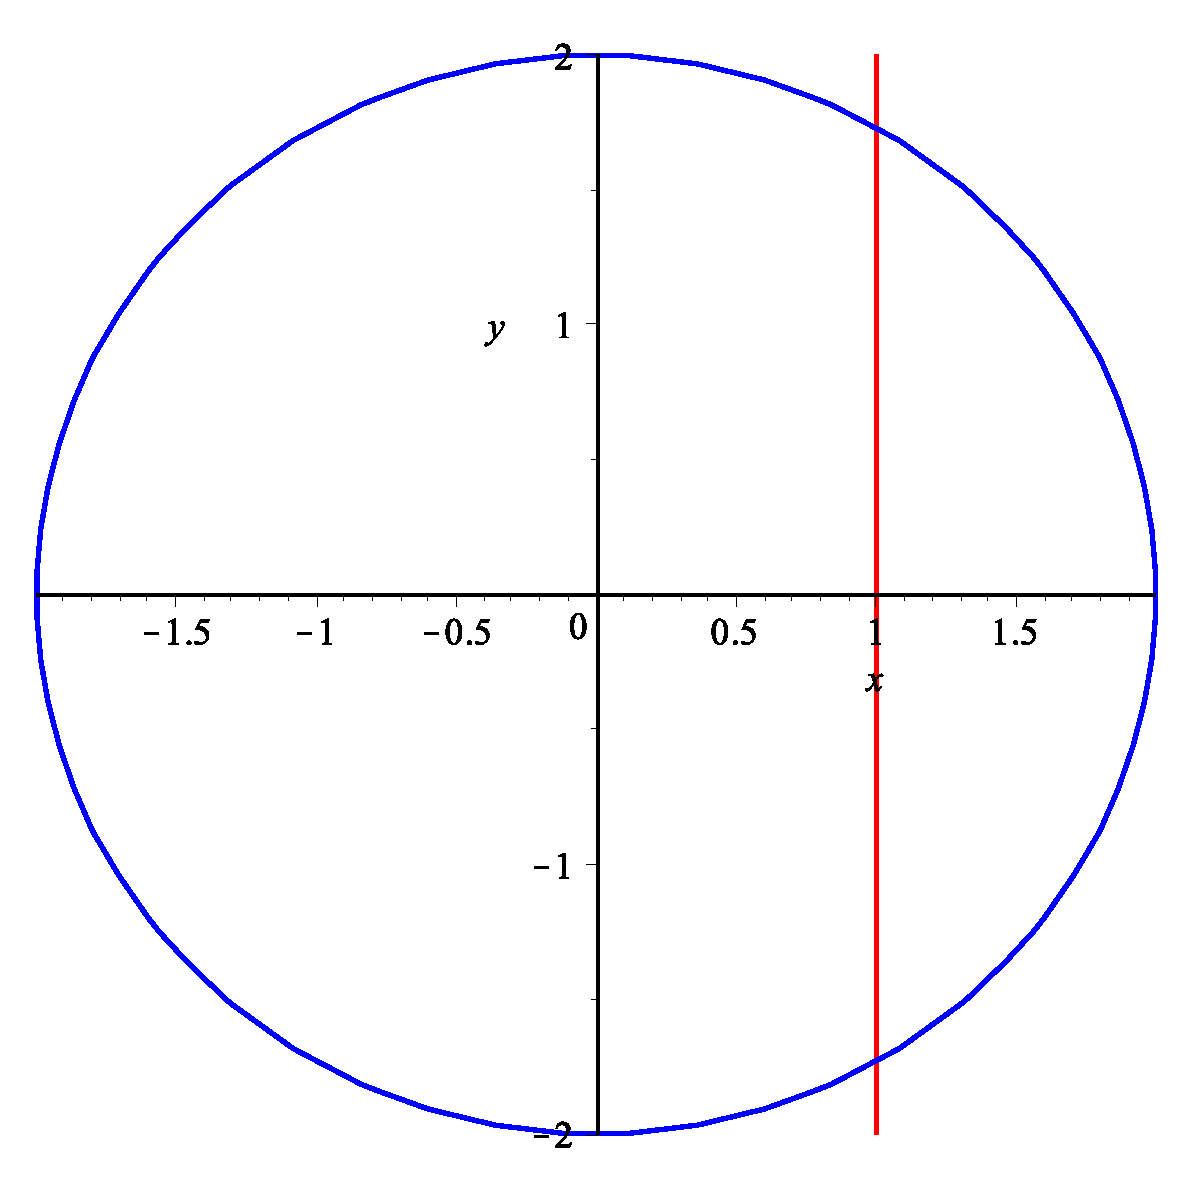
\includegraphics[width=2.5in, height=2.5in]{img/vert_line_test.eps}

\small \textit{Generated with Maple 16} \\
\end{center}

We can see clearly that the vertical line $x=1$ intersects our equation $x^2 + y^2 = 4$ (a circle) at two $y$-values. By the vertical line test, our equation is \textbf{not} a function.

\subsubsection{Manipulation}
\subsubsection{Domain and Range}
\subsubsection{Trigonometry}
\subsubsection{Exercises}

\section{Limits}

\section{Differentiation}

\section{Integration}

\section{Sequences and Series}


\end{document}